\chapter{Numerically stable transport over steep slopes}
\label{ch:cubicFit}

\begin{figure}
	\centering
	\documentclass[tikz]{standalone}
\newcommand{\vect}{\bm}
\newcommand{\Rearth}{R_e}
\newcommand{\lat}{\theta}
\newcommand{\lon}{\lambda}
\newcommand{\transpose}{\intercal}
\newcommand{\sign}{\mathrm{sgn}}
\newcommand{\unitlon}{\bm{\hat{\lon}}}
\newcommand{\unitlat}{\bm{\hat{\lat}}}
\newcommand{\unitk}{\bm{\hat{k}}}
\newcommand{\unitradius}{\bm{\hat{r}}}
\newcommand{\Mag}[1]{\left\lvert #1 \right\rvert}

\begin{document}
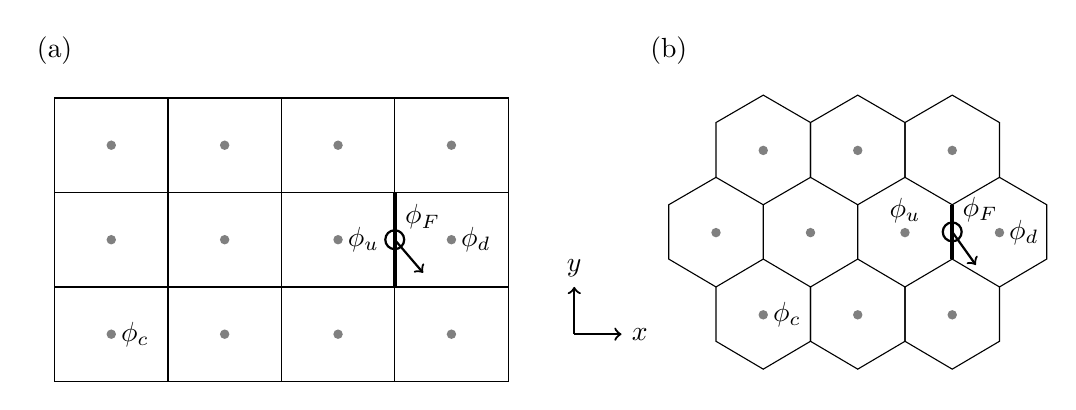
\begin{tikzpicture}[
  scale=0.6,
  cpnt/.style={fill=gray},
]

\begin{scope}[shift={(11,0)}]
	\draw [thick, ->] (0,1) -- (0,2) node [at end, anchor=south] {$y$};
	\draw [thick, ->] (0,1) -- (1,1) node [at end, anchor=west] {$x$};
\end{scope}

\node [above] at (0,6.5) {(a)};
\draw (0,0) rectangle (9.6,6);
\draw (0,2) -- (9.6,2);
\draw (0,4) -- (9.6,4);
\draw (0,0) -- (0,6);
\draw (2.4,0) -- (2.4,6);
\draw (4.8,0) -- (4.8,6);
\draw (7.2,0) -- (7.2,6);

\draw [ultra thick] (7.2,2) -- (7.2,4);
\draw [thick] (7.2,3) circle [radius=0.2] node [anchor=south west] {$\phi_F$};
\draw [thick, ->] (7.2,3) -- (7.8,2.3) node [anchor=west] {$\uf$};

\path [cpnt] (1.2,1) circle [radius=0.1] node [right] {$\phi_c$};
\path [cpnt] (1.2,3) circle [radius=0.1];
\path [cpnt] (1.2,5) circle [radius=0.1];

\path [cpnt] (3.6,1) circle [radius=0.1];
\path [cpnt] (3.6,3) circle [radius=0.1];
\path [cpnt] (3.6,5) circle [radius=0.1];

\path [cpnt] (6.0,1) circle [radius=0.1];
\path [cpnt] (6.0,3) circle [radius=0.1] node [right] {$\phi_u$};
\path [cpnt] (6.0,5) circle [radius=0.1];

\path [cpnt] (8.4,1) circle [radius=0.1];
\path [cpnt] (8.4,3) circle [radius=0.1] node [right] {$\phi_d$};
\path [cpnt] (8.4,5) circle [radius=0.1];

\begin{scope}[shift={(13,2)}]
	\node [above] at (0,4.5) {(b)};

	\draw (1,0) -- (0,0.59) -- (0,1.74) -- (1,2.32) -- (2,1.74) -- (2,0.59) -- (1,0); \path [cpnt] (1,1.15) circle [radius=0.1];
	\draw (2,1.74) -- (3,2.32) -- (4,1.74) -- (4,0.59) -- (3,0) -- (2,0.59); \path [cpnt] (3,1.15) circle [radius=0.1];
	\draw (4,1.74) -- (5,2.32) -- (6,1.74) -- (6,0.59) -- (5,0) -- (4,0.59); \path [cpnt] (5,1.15) circle [radius=0.1] node [above] {$\phi_u$};
	\draw (6,1.74) -- (7,2.32) -- (8,1.74) -- (8,0.59) -- (7,0) -- (6,0.59); \path [cpnt] (7,1.15) circle [radius=0.1] node [right] {$\phi_d$};

	\begin{scope}[shift={(1,-1.74)}]\draw (2,1.74) --(2,0.59) -- (1,0) -- (0,0.59) -- (0,1.74); \path [cpnt] (1,1.15) circle [radius=0.1] node [right] {$\phi_c$};\end{scope}
	\begin{scope}[shift={(3,-1.74)}]\draw (2,1.74) --(2,0.59) -- (1,0) -- (0,0.59) -- (0,1.74); \path [cpnt] (1,1.15) circle [radius=0.1];\end{scope}
	\begin{scope}[shift={(5,-1.74)}]\draw (2,1.74) --(2,0.59) -- (1,0) -- (0,0.59) -- (0,1.74); \path [cpnt] (1,1.15) circle [radius=0.1];\end{scope}

	\begin{scope}[shift={(1,1.74)}]\draw (0,0.59) -- (0,1.74) -- (1,2.32) -- (2,1.74) -- (2,0.59); \path [cpnt] (1,1.15) circle [radius=0.1];\end{scope}
	\begin{scope}[shift={(3,1.74)}]\draw (0,0.59) -- (0,1.74) -- (1,2.32) -- (2,1.74) -- (2,0.59); \path [cpnt] (1,1.15) circle [radius=0.1];\end{scope}
	\begin{scope}[shift={(5,1.74)}]\draw (0,0.59) -- (0,1.74) -- (1,2.32) -- (2,1.74) -- (2,0.59); \path [cpnt] (1,1.15) circle [radius=0.1];\end{scope}

	\draw [ultra thick] (6,0.59) -- (6,1.74);
	\draw [thick] (6,1.165) circle [radius=0.2] node [anchor=south west] {$\phi_F$};
	\draw [thick, ->] (6,1.165) -- (6.5,0.465) node [anchor=west] {$\uf$};
\end{scope}

\end{tikzpicture}
\end{document}

	\caption{Upwind-biased stencils for faces far away from the boundaries of two-dimensional (a) rectangular and (b) hexagon meshes.  The stencil is used to fit a multidimensional polynomial to cell centre values, $\phi_c$, marked by grey circles, in order to approximate the value $\phi_F$ at the face centroid marked by an open circle.  $\phi_u$ and $\phi_d$ are the values at the centroids of the upwind and downwind cells neighbouring the target face, drawn with a heavy line.  The velocity vector $\uf$ is prescribed at face $f$ and determines the choice of stencil at each time-step.}
	\label{fig:cubicFit:interiorStencils}
\end{figure}

The cubicFit scheme approximates the value of the dependent variable at the face, $\phi_F$, using a least-squares fit over a stencil of surrounding known values.
To introduce the approximation method, we will consider how an approximate value is calculated for a face that is far away from the boundaries of a two-dimensional uniform rectangular mesh.
For any mesh, every interior face connects two adjacent cells.  The velocity direction at the face determines which of the two adjacent cells is the upwind cell.  Since the stencil is upwind-biased and asymmetric, two stencils must be constructed for every interior face, and the appropriate stencil is chosen depending on the velocity direction at each face for every time-step.

The upwind-biased stencil for a face $f$ is shown in figure~\ref{fig:cubicFit:interiorStencils}a.  The wind at the face, $\uf$, is blowing from the upwind cell $c_u$ to the downwind cell $c_d$.
To obtain an approximate value at $f$, a polynomial least-squares fit is calculated using the stencil values.
The stencil has \num{4} points in $x$ and \num{3} points in $y$, leading to a natural choice of polynomial that is cubic in $x$ and quadratic in $y$,
\begin{align}
	\phi = a_1 + a_2 x + a_3 y + a_4 x^2 + a_5 xy + a_6 y^2 + a_7 x^3 + a_8 x^2 y + a_9 x y^2 \label{eqn:cubicFit:fullPoly} \text{ .}
\end{align}
A least-squares approach is needed because the system of equations is overconstrained, with \num{12} stencil values but only \num{9} polynomial terms.  The stencil geometry is expressed in a local coordinate system with the face centroid as the origin so that the approximated value $\phi_F$ is equal to the constant coefficient $a_1$.
The stencil is upwind-biased to improve numerical stability, and the multidimensional cubic polynomial is chosen to improve accuracy in the direction of flow \citep{leonard1993}.

The remainder of this \TODO{subsection} generalises the approximation technique for arbitrary meshes and describes the methods for constructing stencils, performing a least-squares fit with a suitable polynomial, and ensuring numerical stability of the transport scheme.

